% Stability of the sensitivity shape (input from ch10_sites.tex, after sec:sites_flux)
\section{How stable is the shape of the flux calibration?}
\label{sec:shape_stability}
For reverberation mapping the level of each spectrum is set by its [O\,{\sc iii}] flux, so the grey part of the
calibration (clouds, slit losses) does not matter. What the calibration must get right is the \textit{shape}: the
relative flux at different wavelengths within an order. We measured it on all 139 standards of the two data sets
with a reference spectrum, all taken through the 2\,arcsec slit: 39 of Feige\,110 at COJ (2026 August 4 to October 8)
and 100 at OGG (12 of Feige\,67, 2025 March 24 to April 7; 20 of GD\,153, May 2 to June 1; 68 of
BD$+28^\circ4211$, June 7 to August 30), and on the narrow lines of the 160 AGN spectra. The scripts are
\texttt{work/scripts/sens\_stability.py}, \texttt{narrow\_line\_ratios.py} and \texttt{make\_shape\_figures.py}.

\paragraph{The response from night to night.} We take each standard's own sensitivity $S$ (the one the pipeline
fits to it, Section~\ref{sec:flux_ensemble}), so its response is $1/S$, and divide it by the median response of its
site, removing the mean of the logarithm in each order (the grey level). The top row of Fig.~\ref{fig:sens_shape}
shows the result. The robust scatter of the shape between nights is 1.8 (blue order) and 2.2 per cent (red order) at
COJ, and 1.2 and 3.4 per cent at OGG, rising to 3--6 per cent at the ends of the orders. It hardly depends on the
conditions: the correlation of the tilt of each response with airmass or seeing is at most 0.37 in absolute value.
There is one slow trend. At COJ the blue-order response at 3700\,\AA{} fell by 4.8 per cent per month relative to
5200\,\AA{}, about 10 per cent over the 65 days (Fig.~\ref{fig:shape_time}, top left), as expected from a mirror
coating that ages. The level of the red order relative to the blue order where they overlap (5000--5400\,\AA) varies
by 4.6 (COJ) and 6.3 per cent (OGG) from night to night. This sets the scatter of the red/blue [O\,{\sc iii}]
ratio (6.2--6.3 per cent; Section~\ref{sec:sites_flux}). It does not affect reverberation mapping, which scales each
order by its own [O\,{\sc iii}], but it limits joining the two orders.

\paragraph{The shape a science spectrum gets.} The direct test calibrates each standard the way a science frame is
calibrated, with the sensitivity of other standards, and divides it by its reference spectrum. Standards of the same
night are left out, and so is the one standard flagged as broken by the quality checks (GD\,153 on 2025 May 25: trace
and profile failed, 39 per cent off in shape). The error is measured in 50\,\AA{} bins outside the telluric bands and
40\,\AA{} around the stellar Balmer lines, after removing its mean in each order. Table~\ref{tab:shape} compares
three choices: the ensemble the pipeline uses (Section~\ref{sec:flux_ensemble}), the nearest other standard alone,
and one fixed sensitivity for the whole instrument configuration (the median of all other standards on the same side
of the OGG mirror recoating). As a floor, a standard calibrated with its own sensitivity still differs from its
reference by 0.23 (blue) and 1.06 per cent (red). In the red order the sensitivity is smooth on 600\,\AA{} scales
(to leave the fringes to the fringe correction), so it does not follow every feature of the reference.

\begin{table}[!htbp]
\centering\small
\caption{Shape error of a standard calibrated as a science frame and divided by its reference spectrum: rms over the
50\,\AA{} bins of each order (mean removed), median over the standards (in brackets, the 90th percentile).
OGG: frames after the mirror recoating; the 12 Feige\,67 before it are calibrated with each other.}
\label{tab:shape}
\begin{tabular}{lcccc}
\toprule
Calibration & \multicolumn{2}{c}{COJ (39)} & \multicolumn{2}{c}{OGG (100)} \\
 & blue & red & blue & red \\
 & \multicolumn{4}{c}{(per cent)} \\
\midrule
Nine nearest standards (pipeline) & 1.30 (3.0) & 1.70 (2.8) & 1.22 (2.5) & 1.92 (4.5) \\
Nearest other night alone & 1.40 (3.6) & 1.77 (3.2) & 1.56 (4.3) & 2.45 (6.3) \\
One sensitivity per configuration & 1.44 (3.4) & 1.61 (2.8) & 1.45 (2.7) & 2.09 (4.6) \\
Own sensitivity (floor) & 0.23 & 1.06 & 0.23 & 1.06 \\
\bottomrule
\end{tabular}
\end{table}

The ensemble of the pipeline is the best or equal to the best choice in every case: a calibrated shape is good to
1.2--1.3 per cent in the blue order and 1.7--1.9 per cent in the red. Between 4000 and 7000\,\AA{} the error is
1.1--1.8 per cent; it rises to 3 per cent at the blue end (3400\,\AA) and to 4--5 per cent beyond 8400\,\AA{}
(Fig.~\ref{fig:sens_shape}, bottom). The ensemble follows the slow trend at COJ, which a fixed sensitivity cannot.
It also absorbs a broken standard: with or without the GD\,153 of May 25 among the calibrating standards, the
ensemble numbers are the same, while any spectrum calibrated with that standard alone would be off by tens of per cent. The pipeline does
not yet leave standards flagged by the quality checks out of the ensemble; it should
(Chapter~\ref{sec:recommendations}).

\begin{figure}[!htbp]
\centering
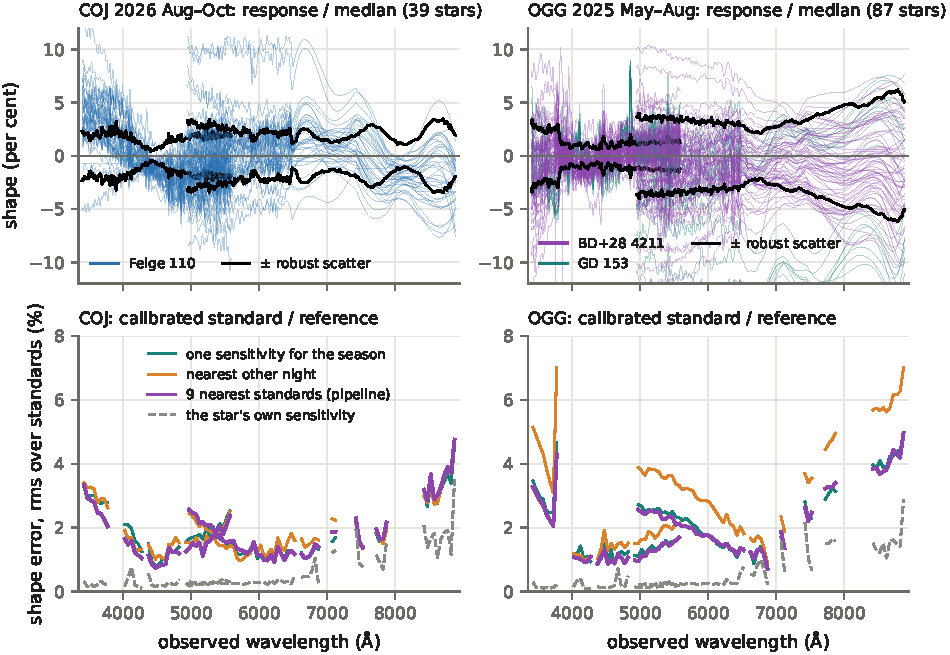
\includegraphics[width=\textwidth]{figures/fig_sens_shape.pdf}
\caption{Stability of the sensitivity shape. Top: the response of each standard divided by the median of its site,
with the mean removed in each order (thin lines, coloured by star; OGG after the mirror recoating); black, plus and
minus the robust scatter. Bottom: the shape error of a standard calibrated as a science frame, divided by its
reference, rms over the standards in 50\,\AA{} bins (telluric bands and stellar Balmer lines left out), for the
three choices of Table~\ref{tab:shape}; dashed, the floor of a standard calibrated with its own sensitivity.}
\label{fig:sens_shape}
\end{figure}

\paragraph{The OGG mirror recoating changed the shape, not only the level.} The throughput step of
Section~\ref{sec:sites_flux} is the re-aluminisation of the primary mirror of Faulkes Telescope North during the
NGC\,4151 campaign. A fresh aluminium coating gains most in the blue, and so does the response
(Fig.~\ref{fig:shape_time}, bottom left): before the recoating, the response at 3400\,\AA{} was 48 per cent lower
relative to 5800\,\AA{} than after it, and at 3700\,\AA{} 32 per cent lower relative to 5200\,\AA. The red order
changed little beyond 6000\,\AA. A sensitivity from after the recoating would therefore put the earlier spectra up to
30 per cent off in shape within the blue order, not just 1.8 times too faint. With the Feige\,67 standards taken before
it, the earlier spectra are calibrated with their own response.

\paragraph{The AGN agree.} The narrow-line region does not vary over months, so the ratio of a narrow line to
[O\,{\sc iii}]\,5007 in the same order tests the calibrated shape without any standard star. We fitted
[O\,{\sc iii}]\,$\lambda\lambda$4959,\,5007 in each order and used its position and width for the other narrow lines,
fitting only their amplitude on a local continuum. In NGC\,4151 (60 spectra over eight months), [O\,{\sc ii}]\,3727 /
[O\,{\sc iii}] scatters by 2.5 per cent and [Ne\,{\sc iii}]\,3869 / [O\,{\sc iii}] by 3.0 per cent, consistent with
the standards plus the measurement noise (Fig.~\ref{fig:shape_time}, bottom right). Before and after the recoating,
[O\,{\sc ii}] / [O\,{\sc iii}] agrees to 0.5 per cent and [Ne\,{\sc iii}] / [O\,{\sc iii}] to 6.6 per cent; the latter
sits on the variable broad H$\epsilon$ and H8 lines. The red/blue [O\,{\sc iii}] ratio was 8 per cent lower before the
recoating, a residual of the older Feige\,67 reference and of the few standards that calibrate that period (all from
its last two weeks). [Ne\,{\sc v}]\,3426 scatters by 8 per cent; the red-order lines ([O\,{\sc i}]\,6300,
[S\,{\sc ii}]\,6716,\,6731) are too weak on the wing of H$\alpha$ to test the shape (15--19 per cent). The narrow lines
of Fairall\,9 are fainter, and the same ratios scatter by about 8 per cent, which is measurement noise.

\begin{figure}[!htbp]
\centering
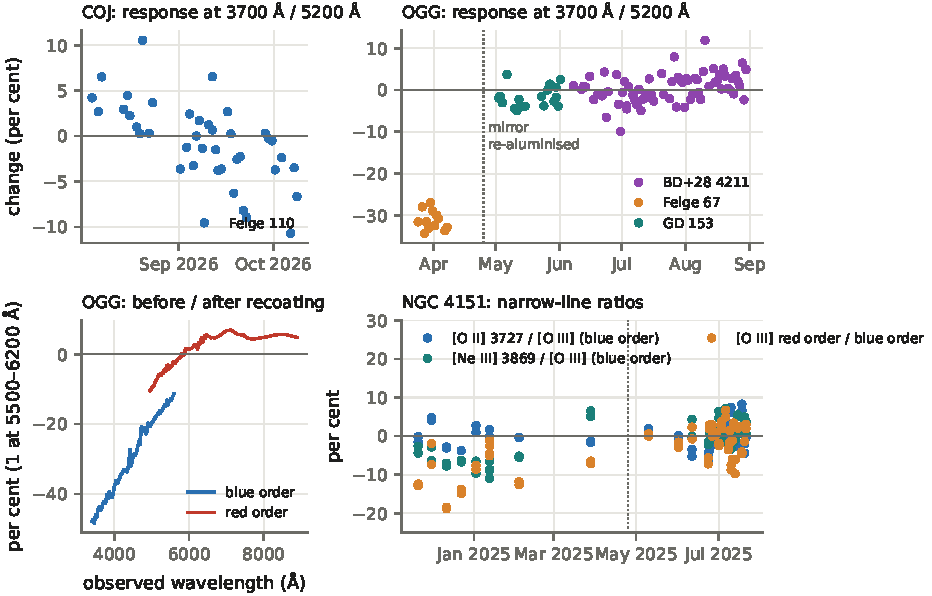
\includegraphics[width=\textwidth]{figures/fig_shape_time.pdf}
\caption{The shape over time. Top: the blue-order response at 3700\,\AA{} relative to 5200\,\AA{} for every standard
at COJ (left) and OGG (right; dotted, the mirror recoating). Bottom left: OGG response before the recoating divided
by the response after it, scaled to 1 at 5500--6200\,\AA. Bottom right: narrow-line ratios of NGC\,4151 divided by
their median after the recoating.}
\label{fig:shape_time}
\end{figure}

\paragraph{In short.} Once [O\,{\sc iii}] sets the level, the shape of a calibrated FLOYDS spectrum is good to about
1--2 per cent between 4000 and 8000\,\AA, 3 per cent at the blue end and 4--5 per cent beyond 8400\,\AA, at both
sites. The response is stable enough from night to night that one sensitivity per instrument configuration would
almost do, but it drifts slowly and jumps when the mirror is recoated. An ensemble of standards near in time, within
one configuration, follows both. Before the OGG recoating, with fewer standards and an older reference, the
blue-order shape is good to 5--8 per cent.
